\documentclass{report}
\usepackage{graphicx} % Required for inserting images
\usepackage[italian]{babel}
\usepackage{tikz}
\usepackage{hyperref}
\usepackage{amsmath}
\usepackage{xcolor}

\definecolor{darkgreen}{rgb}{0.0, 0.5, 0.0}


\title{Protezione e Integrità dei Dati nel Cloud}
\date{Parte V}

\begin{document}

\maketitle

\tableofcontents
\newpage

\chapter{Encryption}
Il \textit{server} potrebbe essere \textbf{\textit{honest-but-curious}}, non dovrebbe 
avere accesso alle risorse; voglio garantire confidenzialità anche rispetto a lui.

Un modo per ottenerla è utilizzare l'\textit{encyption}: si aggiunge 
un livello di protezione attorno ai dati sensibili che li rende non 
leggibili a chi non è autorizzato. 

Di base voglio avere una criptazione dei dati; il problema è il \textbf{bilanciamento tra protezione e funzionalità}, ovvero sulle \textit{query} che è possibile fare sui dati.

\subsubsection{Approcci per accesso a diversi livelli di granularità}

\begin{itemize}
    \item \textbf{\textit{Keyword-based searching:}} passo un \textit{token} già criptato 
    che viene usato per fare ricerca sui dati criptati (voglio trovare dove c'è una certa parola/espressione booleana)
    \begin{figure}[ht]
        \centering
        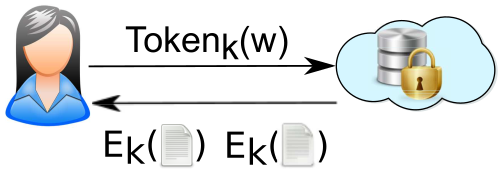
\includegraphics[width=0.4\linewidth]{images/encryption/token-based-search.png}
    \end{figure}
    \item \textbf{Crittografia omomorfica:} crittografia che supporta le operazioni direttamente sul cifrato
    \begin{figure}[ht]
        \centering
        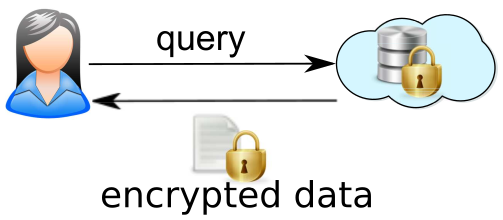
\includegraphics[width=0.4\linewidth]{images/encryption/homomorphic.png}
    \end{figure}
    \item \textbf{\textit{Encryption Schemas:}} ogni colonna può essere cifrata con un diverso schema crittografico 
    (\textit{random, add homomorphic, deterministic, order preserving, \dots})
    \begin{figure}[ht]
        \centering
        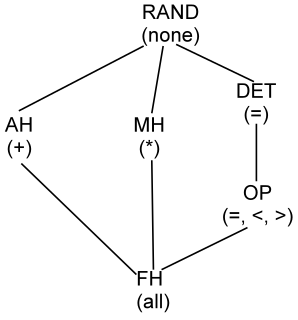
\includegraphics[width=0.3\linewidth]{images/encryption/schemas.png}
    \end{figure}
    \item \textbf{\textit{Onion Encryption:}} cifro i dati con diversi livelli \textit{a cipolla}, ognuno dei quali
    supporta l'esecuzione di una specifica \textit{query SQL}; l'idea è che \textit{scopro il dato solo quando mi serve}
    \begin{figure}[ht]
        \centering
        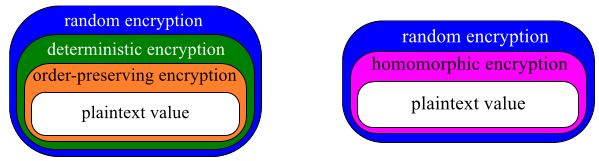
\includegraphics[width=0.8\linewidth]{images/encryption/onion.png}
    \end{figure}
    \item \textbf{Indicizzazione:} associo degli indici ai metadati
    \begin{figure}[ht]
        \centering
        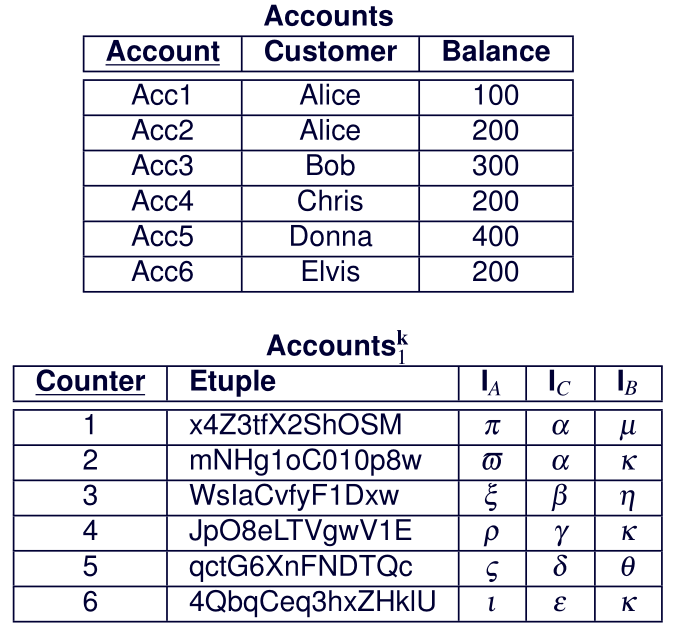
\includegraphics[width=0.6\linewidth]{images/encryption/indicizzazione.png}
    \end{figure}
    Nella seconda tabella: nella seconda colonna c'è la tupla criptata; nelle ultime tre ci sono gli attributi;
    si possono avere diversi tipi di indicizzazione:
    \begin{itemize}
        \item \textbf{\textit{Direct} $(1:1)$}
        
        \textcolor{darkgreen}{\textbf{+}} riesco a fare query precise
        
        \textcolor{red}{\textbf{-}} soggetto ad attacchi di frequenza
        \begin{figure}[ht]
            \centering
            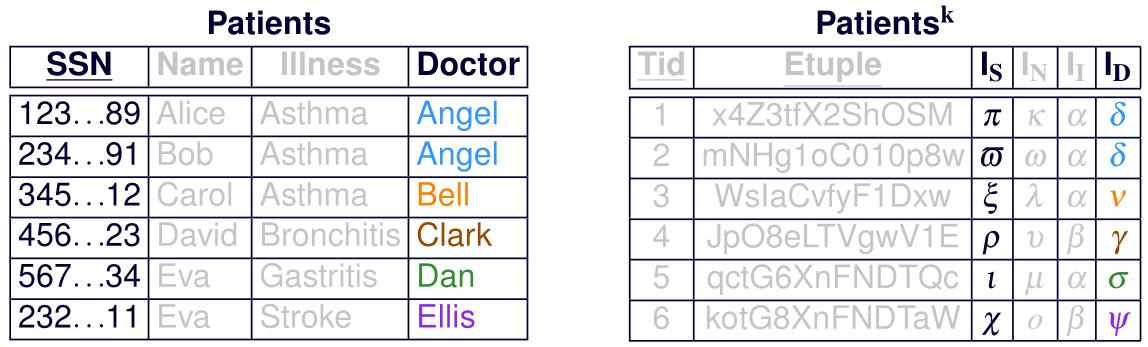
\includegraphics[width=0.85\linewidth]{images/encryption/index-direct.png}
        \end{figure}
        \item \textbf{\textit{Bucket} $(n:1) \rightarrow$} indicizzazione con collisione; ho diversi valori 
        che sono \textbf{mappati allo stesso indice}

        \textcolor{darkgreen}{\textbf{+}} non ho più attacchi di frequenze

        \textcolor{darkgreen}{\textbf{+}} supporta query di uguaglianza (\textit{se un valore è uguale ad un altro})
        
        \textcolor{red}{-} i risultati avranno delle tuple spurie

        \textcolor{red}{-} è ancora possibile fare qualche leakage
        \begin{figure}[ht]
            \centering
            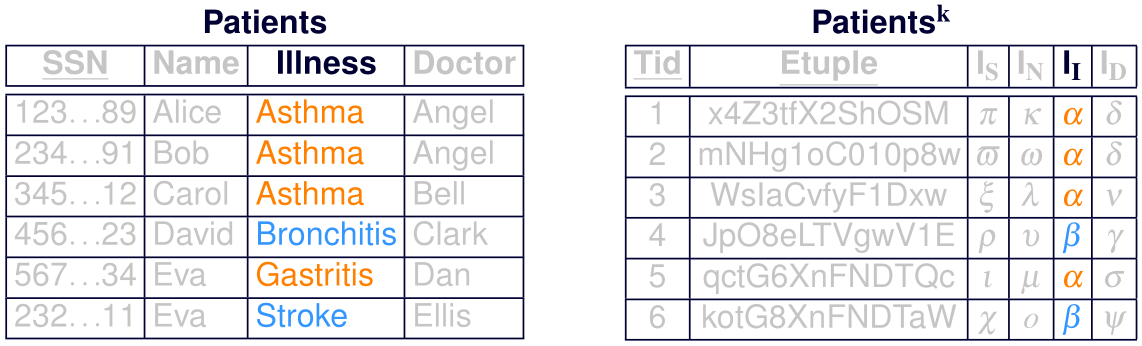
\includegraphics[width=0.85\linewidth]{images/encryption/bucket-index.png}
        \end{figure}
        \textit{In questo caso sono comunque esposto perché asma ha 3 occorrenze, dunque sarà per forza associata ad $\alpha$}

        \item \textbf{\textit{Flattened} $(1:n) \rightarrow$} ciascun indice deve avere lo stesso numero di occorrenze; significa che 
        i valori che hanno più occorrenze sono associati ad indici diversi

        \textcolor{darkgreen}{\textbf{+}} rimuovo la possibilità di fare attacchi di inferenze

        \textcolor{red}{\textbf{-}} sono esposto ad osservazioni dinamiche (magari certi dati sono sempre cercati assieme) 
        \begin{figure}[ht]
            \centering
            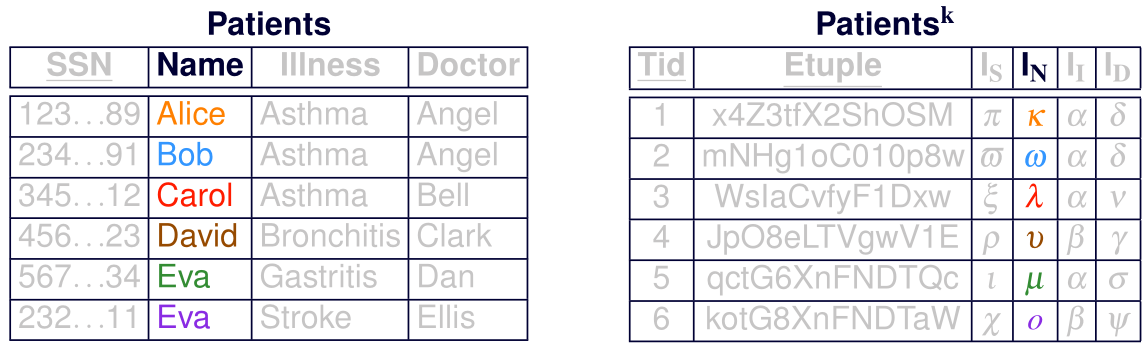
\includegraphics[width=0.85\linewidth]{images/encryption/flattened-index.png}
        \end{figure}

        \item \textbf{\textit{Partition-based:}} 
        
        $\circ$ si partiziona il dominio di un attributo 

        $\circ$ a ciascuna partizione si assegna un'etichetta

        $\circ$ il valore in chiaro viene sostituito dall'etichetta

        \begin{figure}[ht]
            \centering
            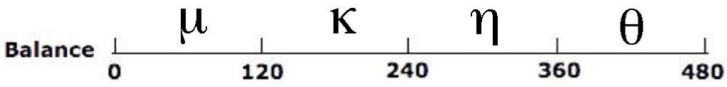
\includegraphics[width=0.6\linewidth]{images/encryption/partion-based-index.png}
        \end{figure}

        \noindent Supporta \textit{query} dove le condizioni sono espressioni booleane del tipo:

        - \textit{Attribute} \texttt{op} \textit{Value}

        - \textit{Attribute} \texttt{op} \textit{Attribute}

        dove \texttt{op}$=\{ =, <, >, \leq, \geq \}$

    \end{itemize}
\end{itemize}











\end{document}